\begin{enumerate}
\item Voici un exemple de pavage d'une grille $3 \times 4$ :

\begin{center}
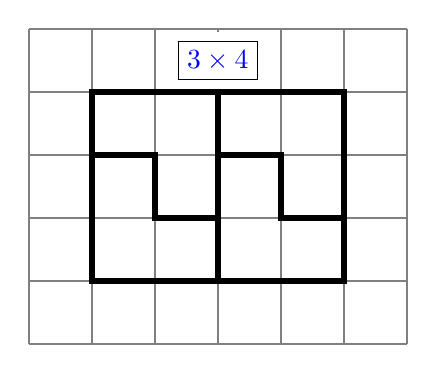
\begin{tikzpicture}[scale=0.8]
    % Dimensions : 10 colonnes (x) et 17 lignes (y)
\def\rows{5}
\def\cols{6}
\def\cell{1} % taille d'une case en cm

% Dessiner la grille grise
\draw[gray, step=\cell, thick] (0,0) grid (\cols*\cell, \rows*\cell);
\draw[line width=2pt, blue] (1,1)--(5,1) -- (5,4) -- (1,4) -- cycle;
\node[fill=white] at (3,4.5) {\fbox{\textcolor{blue}{$3\times 4$}}}; 
\draw[line width=2pt] (1,1)--(3,1) -- (3,2) -- (2,2) -- (2,3) -- (1,3) -- cycle;
\draw[line width=2pt] (1,3)--(1,4) -- (3,4) -- (3,2) ;
\draw[line width=2pt] (3,1)--(5,1) -- (5,2) -- (4,2) -- (4,3) -- (3,3) -- cycle;
\draw[line width=2pt] (3,3)--(3,4) -- (5,4) -- (5,2) ;
\end{tikzpicture}
\end{center}


\item \begin{enumerate}
\item Si une grille $a \times b$ est pavée par des triominos, alors son aire $ab$ est la somme des aires des triominos utilisés. Chaque triomino a une aire égale à $3$. On a donc $3 \mid ab$.

\item Une grille carrée $a \times a$ a pour aire $a^2$. La condition nécessaire est $3 \mid a^2$, donc $3 \mid a$. Le plus petit candidat est donc $a = 3$. \\
La grille $3 \times 3$ n'est pas pavable : le triomino qui recouvre un coin est forcé, il en force un second, et il reste trois cases alignées, ce qui n'est pas un triomino en L. \\
Le candidat suivant est $a = 6$. Une grille $6 \times 6$ se pave en la découpant en six rectangles $2 \times 3$, chacun étant pavable (deux triominos par rectangle). \\
La plus petite grille carrée pavable est donc $\boxed{6 \times 6}$.

\item Non. La condition $3 \mid ab$ n'est pas suffisante : la grille $3 \times 3$ a bien une aire multiple de $3$ mais n'est pas pavable.
\end{enumerate}

\item Pour $a = 2$, la condition nécessaire est $3 \mid 2b$, donc $3 \mid b$. \\
Réciproquement, si $3 \mid b$, on découpe la grille $2 \times b$ en $\frac{b}{3}$ rectangles $2 \times 3$, chacun pavable avec deux triominos. \\
La condition nécessaire et suffisante est donc : \\
$\boxed{\text{La grille } 2 \times b \text{ est pavable si et seulement si } 3 \mid b.}$

\item \begin{enumerate}
\item Après les trois symétries successives, on obtient quatre triominos suivants sur le bandeau $2 \times 16$.

\begin{center}
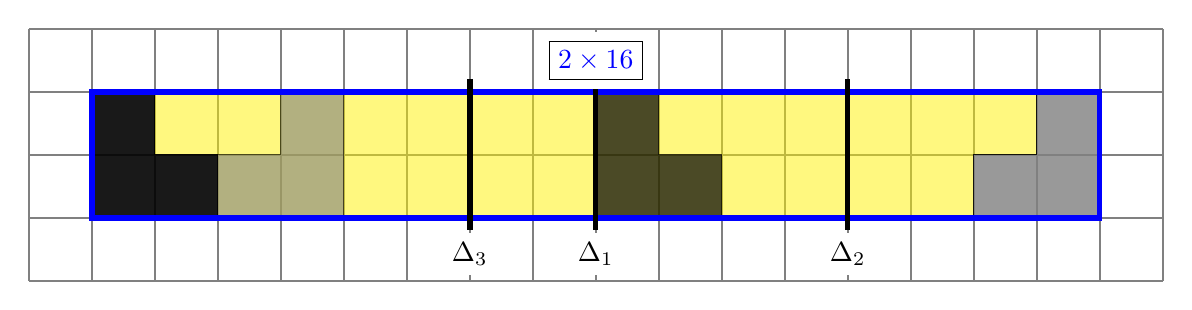
\begin{tikzpicture}[scale=0.8]
    % Dimensions : 10 colonnes (x) et 17 lignes (y)
    \def\rows{4}
    \def\cols{18}
    \def\cell{1} % taille d'une case en cm
    
    % Dessiner la grille grise
    \draw[gray, step=\cell, thick] (0,0) grid (\cols*\cell, \rows*\cell);
    
    % Optionnel : entourer la grille d'un trait plus épais
   % \draw[thick] (0,0) rectangle (\cols*\cell, \rows*\cell); 

\begin{scope}[shift={(2,1)}]
\draw[fill=yellow, opacity=0.5] (0,2) -- (14,2) -- (14,1) -- (13,1) -- (13,0) -- (1,0) -- (1,1) -- (0,1) -- cycle;
\end{scope}

 \begin{scope}[shift={(3,1)}]
 \draw[rotate=90,fill=black, opacity=0.9] (0,0) -- (1,0) -- (1,1) -- (2,1) -- (2,2) -- (0,2) -- cycle;
 \end{scope}
 
 % L n°3 : rotation 180°
 \begin{scope}[shift={(17,3)}]
 \draw[rotate=180,fill=gray, opacity=0.8] (0,0) -- (1,0) -- (1,1) -- (2,1) -- (2,2) -- (0,2) -- cycle;
 \end{scope}
 
 \begin{scope}[shift={(11,1)}]
 \draw[rotate=90,fill=black, opacity=0.7] (0,0) -- (1,0) -- (1,1) -- (2,1) -- (2,2) -- (0,2) -- cycle;
 \end{scope}
 
\begin{scope}[shift={(5,3)}]
\draw[rotate=180,fill=gray, opacity=0.6] (0,0) -- (1,0) -- (1,1) -- (2,1) -- (2,2) -- (0,2) -- cycle;
\end{scope}
  \draw[line width=2pt, blue] (1,1)--(17,1) -- (17,3) -- (1,3) -- cycle;
  
 \draw[line width=2pt, ] (7,3.2)--(7,0.8) node[fill=white,below] {$\Delta_3$};
 
\draw[line width=2pt, ] (9,3.2)--(9,0.8) node[fill=white,below] {$\Delta_1$};

\draw[line width=2pt, ] (13,3.2)--(13,0.8) node[fill=white,below] {$\Delta_2$};

\node[fill=white] at (9,3.5) {\fbox{\textcolor{blue}{$2\times 16$}}};
\end{tikzpicture}
\end{center}

\item Chaque pliage remplace une symétrie par une superposition. Après le premier pliage, on a 2 épaisseurs ; après le deuxième, 4 ; après le troisième, 8. Le triomino noir restant visible, le découpage selon son contour traverse donc 8 épaisseurs identiques, ce qui produit $2^3 = 8$ triominos identiques. Le deuxième bandeau fonctionne exactement de la même façon.
\end{enumerate}

\item \begin{enumerate}
\item Un pavage possible d'une grille $5 \times 6$ :

\begin{center}
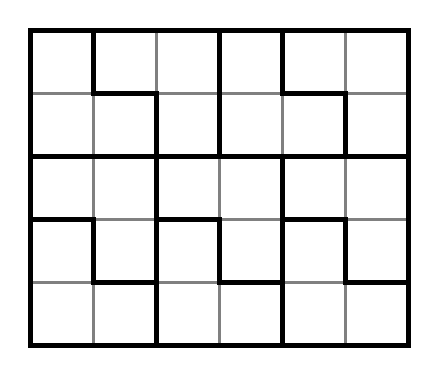
\begin{tikzpicture}[scale=0.8]
    % Dimensions : 10 colonnes (x) et 17 lignes (y)
\def\rows{6}
\def\cols{7}
\def\cell{1} % taille d'une case en cm

% Dessiner la grille grise
\draw[gray, step=\cell, thick] (1,1) grid (\cols*\cell, \rows*\cell);
\draw[line width=2pt, blue] (1,1)--(7,1) -- (7,6) -- (1,6) -- cycle;
%\node[fill=white] at (4,6.5) {\fbox{\textcolor{blue}{$5\times 6$}}}; 
\draw[line width=2pt] (1,1)--(3,1) -- (3,2) -- (2,2) -- (2,3) -- (1,3) -- cycle;
\draw[line width=2pt] (1,3)--(1,4) -- (3,4) -- (3,2) ;
\draw[line width=2pt] (3,1)--(5,1) -- (5,2) -- (4,2) -- (4,3) -- (3,3) -- cycle;
\draw[line width=2pt] (3,3)--(3,4) -- (5,4) -- (5,2) ;
\draw[line width=2pt] (5,1)--(7,1) -- (7,2) -- (6,2) -- (6,3) -- (5,3) -- cycle;
\draw[line width=2pt] (5,3)--(5,4) -- (7,4) -- (7,2) ;
\draw[line width=2pt] (1,4)--(3,4) -- (3,5) -- (2,5) -- (2,6) -- (1,6) -- cycle;
\draw[line width=2pt] (2,5)--(2,6) -- (4,6) -- (4,4) ;
\draw[line width=2pt] (4,4)--(6,4) -- (6,5) -- (5,5) -- (5,6) -- (4,6) -- cycle;
\draw[line width=2pt] (5,5)--(5,6) -- (7,6) -- (7,4) ;
\end{tikzpicture}
\end{center}
\newpage
\item Un pavage possible d'une grille $5 \times 9$ :

\begin{center}
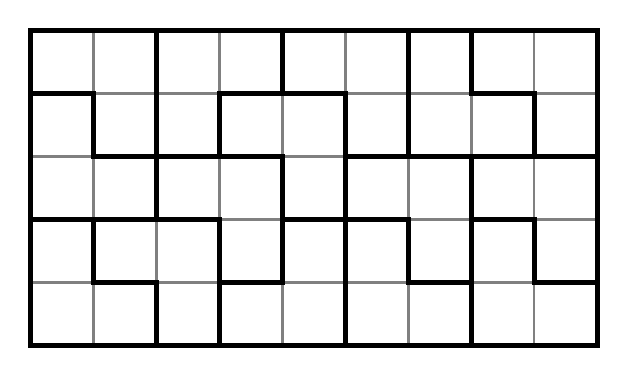
\begin{tikzpicture}[scale=0.8]
    % Dimensions : 10 colonnes (x) et 17 lignes (y)
\def\rows{6}
\def\cols{10}
\def\cell{1} % taille d'une case en cm

% Dessiner la grille grise
\draw[gray, step=\cell, thick] (1,1) grid (\cols*\cell, \rows*\cell);
\draw[line width=2pt] (1,1)--(10,1) -- (10,6) -- (1,6) -- cycle;
%\node[fill=white] at (4,6.5) {\fbox{\textcolor{blue}{$5\times 6$}}}; 
\draw[line width=2pt] (1,1)--(3,1) -- (3,2) -- (2,2) -- (2,3) -- (1,3) -- cycle;
\draw[line width=2pt] (2,3)--(4,3) -- (4,1) -- (3,1) ;
\draw[line width=2pt] (1,3)--(3,3) -- (3,4) -- (2,4) -- (2,5) -- (1,5) -- cycle;
\draw[line width=2pt] (1,5)--(1,6) -- (3,6) -- (3,4) ;
\draw[line width=2pt] (6,1)--(8,1) -- (8,2) -- (7,2) -- (7,3) -- (6,3) -- cycle;
\draw[line width=2pt] (3,4)--(5,4) -- (5,2) -- (4,2) ;
\draw[line width=2pt] (8,1)--(10,1) -- (10,2) -- (9,2) -- (9,3) -- (8,3) -- cycle;
\draw[line width=2pt] (4,4) -- (4,5)--(6,5) -- (6,3) -- (5,3) ;
\draw[line width=2pt] (5,5) -- (5,6)--(7,6) -- (7,4) -- (6,4) ;
\draw[line width=2pt] (7,4)--(9,4) -- (9,5) -- (8,5) -- (8,6) -- (7,6) -- cycle;
\draw[line width=2pt] (8,3)--(8,4) -- (10,4) ;
\end{tikzpicture}
\end{center}

\item Soit $b$ un multiple de $3$ avec $b \geqslant 6$. Alors $b$ est de la forme $6k$ ou $6k+3$ ($k\geqslant 1$). \\
Si $b = 6k$, on juxtapose $k$ grilles $5 \times 6$. \\
Si $b = 6k+3$, on juxtapose $(k-1)$ grilles $5 \times 6$ et une grille $5 \times 9$. \\
Ainsi, pour tout $b \geqslant 6$ multiple de $3$, la grille $5 \times b$ est pavable.
\end{enumerate}

\item On suppose $b$ multiple de $3$ et qu'une grille $a \times b$ est pavable. D'après la question 3, une grille $2 \times b$ est également pavable. En accolant à la grille $a \times b$ une bande $2 \times b$, on obtient un pavage de la grille $(a+2) \times b$. Donc :
\[
a \times b \text{ pavable } \implies (a+2) \times b \text{ pavable, dès que } 3 \mid b.
\]

\item La nécessité a déjà été vue en 2.(a) : si la grille $a \times b$ est pavable, alors $3 \mid ab$. \\
Réciproquement, supposons $a \geqslant 4$, $b \geqslant 4$ et $3 \mid ab$. Par symétrie, on peut supposer $3 \mid b$ (si ce n'est pas le cas, $3 \mid a$ et on échange les rôles). Comme $b \geqslant 4$ et $3 \mid b$, on a en fait $b \geqslant 6$. \\
— Si $a$ est pair, on part d'une grille $2 \times b$ (pavable d'après la question 3), puis on applique plusieurs fois la question 6 pour obtenir successivement $4 \times b$, $6 \times b$, ..., jusqu'à $a \times b$. \\
— Si $a$ est impair, alors $a \geqslant 5$. On part d'une grille $5 \times b$ (pavable d'après la question 5.c), puis on applique plusieurs fois la question 6 pour atteindre $a \times b$. \\
On a donc démontré :
\[
\boxed{\text{Pour } a, b \geqslant 4,\quad a \times b \text{ est pavable } \iff 3 \mid ab.}
\]
Pour une grille carrée $a \times a$ avec $a \geqslant 4$, cela devient :
\[
a \times a \text{ pavable } \iff 3 \mid a^2 \iff 3 \mid a.
\]
En tenant compte de la question 2.(b) (la grille $3 \times 3$ n'est pas pavable), les grilles carrées pavables sont exactement :
\[
\boxed{a \times a \text{ avec } a \geqslant 6 \text{ et } 3 \mid a.}
\]
\end{enumerate}
